\documentclass[
11pt, % The default document font size, options: 10pt, 11pt, 12pt
%codirector, % Uncomment to add a codirector to the title page
]{charter} 


% El títulos de la memoria, se usa en la carátula y se puede usar el cualquier lugar del documento con el comando \ttitle
\titulo{Sistema de monitoreo de calidad del aire} 

% Nombre del posgrado, se usa en la carátula y se puede usar el cualquier lugar del documento con el comando \degreename
%\posgrado{Carrera de Especialización en Sistemas Embebidos} 
\posgrado{Carrera de Especialización en Internet de las Cosas} 
%\posgrado{Carrera de Especialización en Inteligencia Artificial}
%\posgrado{Maestría en Sistemas Embebidos} 
%\posgrado{Maestría en Internet de las cosas}

% Tu nombre, se puede usar el cualquier lugar del documento con el comando \authorname
% IMPORTANTE: no omitir titulaciones ni tildación en los nombres, también se recomienda escribir los nombres completos (tal cual los tienen en su documento)
\autor{Ing. Rodrigo Jurgen Pinedo Nava}

% El nombre del director y co-director, se puede usar el cualquier lugar del documento con el comando \supname y \cosupname y \pertesupname y \pertecosupname
\director{Por definir}
\pertenenciaDirector{pertenencia} 
\codirector{} % para que aparezca en la portada se debe descomentar la opción codirector en los parámetros de documentclass
\pertenenciaCoDirector{FIUBA}

% Nombre del cliente, quien va a aprobar los resultados del proyecto, se puede usar con el comando \clientename y \empclientename
\cliente{Ing. Jose Mauricio Vargas Nuñez}
\empresaCliente{Alicorp}
 
\fechaINICIO{4 de marzo de 2025}		%Fecha de inicio de la cursada de GdP \fechaInicioName
\fechaFINALPlan{22 de abril de 2025} 	%Fecha de final de cursada de GdP
\fechaFINALTrabajo{octubre de 2025}	%Fecha de defensa pública del trabajo final

\usepackage[spanish]{babel}
\addto\captionsspanish{\renewcommand{\tablename}{Tabla}}



\begin{document}

\maketitle
\thispagestyle{empty}
\pagebreak

\thispagestyle{empty}
{\setlength{\parskip}{0pt}
\tableofcontents{}
}
\pagebreak


\section*{Registros de cambios}
\label{sec:registro}


\begin{table}[ht]
\label{tab:registro}
\centering
\begin{tabularx}{\linewidth}{@{}|c|X|c|@{}}
\hline
\rowcolor[HTML]{C0C0C0} 
Revisión & \multicolumn{1}{c|}{\cellcolor[HTML]{C0C0C0}Detalles de los cambios realizados} & Fecha      \\ \hline
0      & Creación del documento                                 &\fechaInicioName \\ \hline
1      & Se completa hasta el punto 5 inclusive                 & 20 de marzo de 2025 \\ \hline
2      & Se completa hasta el punto 9 inclusive                 & 28 de marzo de 2025 \\ \hline
3      & Se completa hasta el punto 11 inclusive                 & 4 de abril de 2025 \\ \hline
%1      & Se completa hasta el punto 5 inclusive                & {día} de {mes} de 202X \\ \hline
%2      & Se completa hasta el punto 9 inclusive
%		  Se puede agregar algo más \newline
%		  En distintas líneas \newline
%		  Así                                                    & {día} de {mes} de 202X \\ \hline
%3      & Se completa hasta el punto 12 inclusive                & {día} de {mes} de 202X \\ \hline
%4      & Se completa el plan	                                 & {día} de {mes} de 202X \\ \hline

% Si hay más correcciones pasada la versión 4 también se deben especificar acá

\end{tabularx}
\end{table}

\pagebreak



\section*{Acta de constitución del proyecto}
\label{sec:acta}

\begin{flushright}
Buenos Aires, \fechaInicioName
\end{flushright}

\vspace{2cm}

Por medio de la presente se acuerda con el \authorname\hspace{1px} que su Trabajo Final de la \degreename\hspace{1px} se titulará ``\ttitle'' y consistirá en {la implementación de una red de sensores especializados para la medición de partículas en suspensión, dióxido de carbono, compuestos orgánicos volátiles, temperatura y humedad ambiental para la recopilación y transmisión de datos en tiempo real}. El trabajo tendrá un presupuesto preliminar estimado de {600} horas y un costo estimado de {\$ 500}, con fecha de inicio el \fechaInicioName\hspace{1px} y fecha de presentación pública en \fechaFinalName.

Se adjunta a esta acta la planificación inicial.

\vfill

% Esta parte se construye sola con la información que hayan cargado en el preámbulo del documento y no debe modificarla
\begin{table}[ht]
\centering
\begin{tabular}{ccc}
\begin{tabular}[c]{@{}c@{}}Dr. Ing. Ariel Lutenberg \\ Director posgrado FIUBA\end{tabular} & \hspace{2cm} & \begin{tabular}[c]{@{}c@{}}\clientename \\ \empclientename \end{tabular} \vspace{2.5cm} \\ 
\multicolumn{3}{c}{\begin{tabular}[c]{@{}c@{}} \supname \\ Director del Trabajo Final\end{tabular}} \vspace{2.5cm} \\
\end{tabular}
\end{table}




\section{1. Descripción técnica-conceptual del proyecto a realizar}
\label{sec:descripcion}

La contaminación del aire es un problema crítico que afecta tanto a entornos urbanos como industriales, con consecuencias directas sobre la salud pública y el medio ambiente. En Argentina, la situación es alarmante. Según la Organización Mundial de la Salud (OMS), el aire en el país tiene una media anual de 13 µg/m³ de partículas PM2.5, superando en un 30\% el nivel considerado seguro por la organización. En Buenos Aires, esta media anual asciende a 14 µg/m³, lo que implica un 40\% por encima del límite recomendado. Estas cifras se traducen en consecuencias graves, como la muerte anual de 85 niños por enfermedades vinculadas a la contaminación del aire en Argentina.

Este proyecto nace como un emprendimiento personal con el propósito de monitorear la calidad del aire en entornos industriales y urbanos y proporcionar información clave para la toma de decisiones. Actualmente, muchas ciudades y empresas carecen de sistemas eficientes y accesibles para medir en tiempo real la calidad del aire, lo que dificulta la prevención y el control de la contaminación. El objetivo es llenar ese vacío con una solución tecnológica asequible y escalable.

Se propone desarrollar un sistema de monitoreo basado en una red de sensores y la tecnología internet de las cosas (IoT). El sistema será capaz de detectar partículas en el aire tales como PM2.5, niveles de CO2, compuestos químicos dañinos, temperatura y humedad. Los datos obtenidos serán enviados a una plataforma accesible desde un aplicativo web. Los dispositivos estarán conectados mediante LoRaWAN y WiFi/MQTT, almacenarán datos de manera eficiente y se presentarán en una plataforma intuitiva. Revisar la Figura 1 para comprender el diagrama de bloques del sistema de monitoreo.

\begin{figure}[htpb]
\centering 
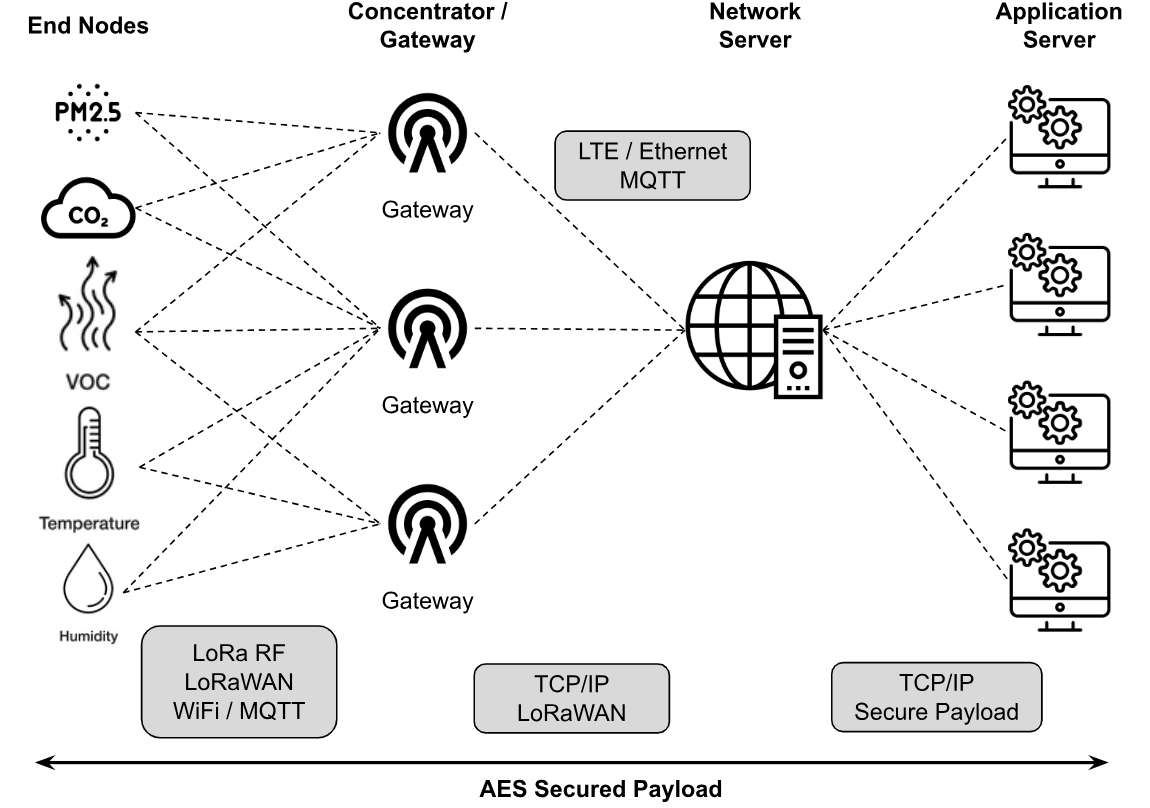
\includegraphics[width=.65\textwidth]{./Figuras/fig_1-diagBloques.png}
\caption{Diagrama en bloques del sistema.}
\label{fig:diagBloques}
\end{figure}

Este proyecto está diseñado como una solución adaptable, principalmente para implementarse en empresas, con la capacidad de escalar a hogares y gobiernos. Todos los usuarios comparten una preocupación en común, la calidad del aire y su impacto en la salud. El sistema no solo permite el monitoreo en tiempo real, sino también envía alertas cuando los niveles de contaminación superan los límites recomendados. También ofrece herramientas para analizar datos históricos e identificar tendencias, que permitan tomar decisiones oportunas. Más que una simple innovación tecnológica, este proyecto representa una herramienta clave para mejorar la calidad de vida y promover un entorno más saludable y sostenible.

En el mercado actual existen soluciones para el monitoreo de la calidad del aire, sin embargo, muchas de ellas presentan limitaciones, como pueden ser:
\begin{itemize}
	\item Costos elevados: en las etapas de implementación y mantenimiento, un sistema con carácteristicas similares puede volverse solo accesible a instituciones con grandes presupuestos.
	\item Cobertura limitada: debido a que la mayoría de los sensores requieren cableado o dependencias de redes WiFi con alcance reducido.
	\item Falta de integración con plataformas acceesibles: lo que dificulta el análisis y la interpretación de los datos por parte de usuarios sin conocimientos técnicos avanzados.
\end{itemize}

A diferencia de las soluciones mencionadas, este proyecto estará diseñado como una solución flexible y adaptable a  empresas, hogares y gobiernos. Su propuesta de valor se basa en ofrecer un monitoreo ambiental accesible, para lograr entornos seguros y sostenibles, bajo los siguientes aspectos:

\begin{itemize}
	\item Accesibilidad: una solución asequible en comparación con otros sistemas comerciales.
	\item Escalabilidad: implementación modular, adaptable a distintos entornos y necesidades.
	\item Interfaz intuitiva: plataforma accesible para cualquier usuario, sin necesidad de conocimientos técnicos avanzados.
	\item Conectividad eficiente: uso de tecnologías de comunicación de bajo consumo y gran alcance.
	\item Toma de decisiones informada: alertas y análisis de datos para implementar medidas de mitigación de contaminación.
\end{itemize}

El proyecto se encuentra en una etapa inicial de desarrollo. Para su primera versión se plantea una solución funcional, enfocada en validar su desempeño en entornos reales. En esta fase, el sistema ofrecerá dos modalidades de monitoreo que permitirán a los usuarios gestionar sus dispositivos de manera flexible:  

\begin{itemize}
    \item Monitoreo privado: cada usuario podrá registrar y gestionar sus propios dispositivos, accediendo a la información en tiempo real de los sensores vinculados.  
    \item Monitoreo público: si el usuario así lo decide, podrá compartir los datos recopilados con la comunidad, permitiendo que la información esté disponible en una red abierta. Esto fomentará la creación de un ecosistema colaborativo.  
\end{itemize}

En esta primera versión no se implementarán modelos de suscripción ni esquemas de pago, ya que el objetivo principal es desarrollar un prototipo funcional. Este proyecto permitirá evaluar la viabilidad técnica y el impacto del sistema en distintos escenarios de uso.  

A futuro se integrará inteligencia artificial (IA) para análisis predictivo y se aumentarán funcionalidades para mejorar la toma de decisiones urbanas e industriales. El proyecto busca un crecimiento accesible y escalable, garantizando que cada usuario se beneficien de un monitoreo ambiental confiable desde su primera versión.



\vspace{25px}


\section{2. Identificación y análisis de los interesados}
\label{sec:interesados}

\begin{table}[ht]
%caption{Identificación de los interesados}
%\label{tab:interesados}
\begin{tabularx}{\linewidth}{@{}|*{4}{>{\arraybackslash}X|}@{}}
\hline
\rowcolor[HTML]{C0C0C0} 
Rol           & Nombre y Apellido & Organización 	& Puesto 	\\ \hline
% Auspiciante   & -                 & -             	& -       	\\ \hline
Cliente       & \clientename      &\empclientename	& Supervisor de Almacén       	\\ \hline
% Impulsor      & -                 & -             	& -       	\\ \hline
Responsable   & \authorname       & FIUBA        	& Alumno 	\\ \hline
% Colaboradores & -                 & -             	& -       	\\ \hline
Orientador    & \supname	      & \pertesupname 	& Director del Trabajo Final \\ \hline
Usuario final & Industrias, hogares o gobiernos	&  Privada o pública & 		\\
\hline
% Equipo        & -                 & -             	& -       	\\ \hline
\end{tabularx}
\end{table}

\begin{itemize}
	\item Cliente: el Ing. Jose Mauricio Vargas Nuñez es quien propuso los requerimientos del proyecto.
	\item Orientador: \supname es un profesional idóneo para la temática con especialidad en tecnologías IoT y LoRaWAN.
\end{itemize}

\section{3. Propósito del proyecto}
\label{sec:proposito}

El propósito de este proyecto es fomentar entornos más saludables, seguros y sostenibles en zonas urbanas e industriales, a partir de una mejora en la calidad del aire. Esto se logrará mediante un sistema de monitoreo basado en IoT, que permita recopilar, analizar y visualizar datos ambientales en tiempo real. Con esta herramienta, se busca facilitar la identificación de fuentes de contaminación y alertar para que las partes interesadas tomen acciones correctivas oportunas. Además, se busca que la solución sea escalable, accesible y eficiente, lo que asegurará su adaptabilidad a distintos entornos y necesidades.

\section{4. Alcance del proyecto}
\label{sec:alcance}

Este proyecto abarca el desarrollo e implementación de un sistema de monitoreo de calidad del aire basado en IoT. El sistema será capáz de medir, transmitir, almacenar y mostrar datos en tiempo real, proporcionando información clave para la toma de decisiones.

El proyecto incluye:

\begin{itemize}
	\item Sensores para medir partículas en suspensión, dióxido de carbono, compuestos orgánicos volátiles, temperatura y humedad.
	\item Microcontrolares ESP32 con modulo LoRa y antena para una comunicación con el servidor mediante protocolos de LoRaWAN, WiFi, MQTT y TCP/IP.
	\item Servidor AWS IoT Core, usando \textit{brocker} Mosquito y el diseño de la base de datos SQL/NoSQL con PostgreSQL.
	\item El diseño de una aplicación web para las visualizaciones del usuario, donde se verán los dispositivos conectados, mediciones, gráficas de históricos y alertas.
	
	
\end{itemize}

El presente proyecto no incluye:
\begin{itemize}
	\item Desarrollo de modelos de suscripción o monetización, ya que en esta fase el enfoque es la validación del prototipo.
	\item Integración con inteligencia artificial o modelos predictivos avanzados.
	\item Implementación de una red de sensores a gran escala más allá del piloto inicial.
	\item Certificaciones oficiales de calidad del aire, ya que el sistema servirá como referencia complementaria a mediciones gubernamentales o institucionales.
	\item Localización geográfica que marque el estado de las zonas monitoreadas.
\end{itemize}

El alcance del proyecto está limitado a ser considerado un prototipo, enfocado en validar la viabilidad técnica y operativa. Las futuras versiones podrán incorporar mejoras basadas en los resultados de esta etapa.

\section{5. Supuestos del proyecto}
\label{sec:supuestos}

Para el desarrollo del presente proyecto se supone que:

\begin{itemize}
	\item Disponibilidad financiera: dado que se trata de un emprendimiento personal, los costos del proyecto podrán ser cubiertos por el responsable del proyecto.
	\item Disponibilidad tecnológica: se contará con acceso a los sensores, microcontroladores y todos los componentes necesarios para la fabricación de los dispositovos IoT.
	\item Tiempo: el responsable cumplirá con la planificación propuesta, evitará retrasos y culminará el proyecto de manera satisfactoria.
	\item Infraestructura de comunicación: podrán realizarse pruebas en entornos controlados pertinentes para el correcto desarrollo del proyecto.
	\item Servidores cloud: se contará con espacios de prueba en AWS, los dominios y servicios para utilizar el \textit{brocker} Mosquito.

\end{itemize}

\section{6. Requerimientos}
\label{sec:requerimientos}

\begin{enumerate}

	\item Requerimientos funcionales:
	\begin{enumerate}
	

		\item El sistema permitirá la captura periódica de datos ambientales a través de sensores conectados a dispositivos IoT.
		\item Los datos se transmitirán al servidor en tiempo real utilizando LoRaWAN o WiFi/MQTT según el entorno.
		\item El sistema deberá almacenar los datos para su posterior análisis.
		\item Se deberá ofrecer la opción de publicar los datos de manera privada o pública.
		\item La interfaz será capaz de mostrar a los usuarios las mediciones de sus dispositivos y las zonas que tenga registrado un usuario.
		\item Deberá generarse una alerta cuando los valores superen los umbrales definidos como peligrosos.
	\end{enumerate}
	
	\item Requerimientos de infraestructura
	\begin{enumerate}
		\item Se deberá contar con acceso a una red WiFi estable o cobertura LoRaWAN en las zonas de instalación de los dispositivos.
		\item El sistema requerirá un servidor local o en la nube con capacidad para recibir, procesar y almacenar datos provenientes de múltiples nodos.
		\item La base de datos utilizada deberá estar optimizada para el manejo de series temporales y para la gestión estructurada de usuarios y configuraciones.
		\item La alimentación de los dispositivos deberá realizarse mediante batería recargable o fuente USB, con posibilidad de alimentación solar para aplicaciones en exteriores.	
	\end{enumerate}
	
	\item Requerimientos de documentación
	\begin{enumerate}
		\item Deberá documentarse el proceso de montaje del hardware, incluyendo la conexión de sensores al microcontrolador ESP32-S3 y la configuración de red.
		\item Se deberá incluir un manual de instalación y uso de la plataforma web.
		\item La documentación deberá contemplar las APIs utilizadas o desarrolladas para la comunicación entre dispositivos y servidor.	
	\end{enumerate}

	\item Requerimientos del entregable
	\begin{enumerate}
		\item El entregable consistirá en un prototipo funcional que incluya al menos dos dispositivos que realicen las mediciones ambientales, un nodo IoT operativo, una plataforma web de visualización, un sistema de almacenamiento de datos y un módulo de alertas.
		\item El sistema deberá estar probado en un entorno controlado y documentado como prueba de concepto.
		\item Se desarrollará la memoria final del proyecto.

	\end{enumerate}
	
	\item Requerimientos de la interfaz
	\begin{enumerate}
		\item La plataforma deberá contar con una interfaz web responsiva para el monitoreo.
		\item La interfaz permitirá visualizar datos en tiempo real, acceder a históricos, gestionar dispositivos y configurar alertas.
		\item Los indicadores de calidad del aire deberán representarse mediante códigos de colores intuitivos y comprensibles.
		\item El sistema ofrecerá una interfaz de visualización con lecturas de datos ambientales de las zonas definidas como públicas. Se limitará la visualización al estado de las zonas sin tener acceso a los dispositivos vinculados y datos históricos.

	\end{enumerate}

	\item Requerimientos funcionales del sistema para el rol “usuario”
	\begin{enumerate}
		\item El usuario deberá poder registrarse y asociar dispositivos a su cuenta personal.
		\item El usuario gestionará sus dispositivos pudiendo agregar, eliminar, editar y asignar la ubicación en zonas definidas.
		\item Tendrá acceso a la visualización en tiempo real de los datos capturados por sus sensores.
		\item Podrá decidir si desea compartir sus datos de forma pública o mantenerlos en modo privado.
		\item Recibirá alertas personalizadas cuando los valores medidos superen los umbrales definidos.

	\end{enumerate}

	\item Requerimientos funcionales del sistema para el rol “administrador”
	\begin{enumerate}
		\item El administrador deberá tener acceso a la gestión de usuarios, dispositivos y configuraciones generales del sistema.
		\item Tendrá visibilidad completa sobre las métricas generadas por todos los nodos activos.
		\item Deberá poder acceder a registros \textit{(logs)} del sistema y supervisar el estado de funcionamiento de cada dispositivo.

	\end{enumerate}

	\item Requerimientos funcionales del sistema para la vista pública
	\begin{enumerate}
		\item La persona que quiera tener acceso a la vista pública deberá llenar un formulario donde se exprese su intención de acceder a esta información.
		\item La interfaz pública tendrá a disposición el estado en tiempo real de las mediciones ambientales de las zonas públicas.

	\end{enumerate}

	\item Requerimientos de seguridad
	\begin{enumerate}
		\item El sistema gestionará las credenciales para el ingreso de los usuarios.
		\item Se contará con métodos para recuperación de contraseñas y verificación de usuarios.
		\item La información asociada a los usuarios y a dispositivos configurados como privados deberá mantenerse protegida y no podrá hacerse pública sin consentimiento expreso.

	\end{enumerate}

\end{enumerate}

\section{7. Historias de usuarios (\textit{Product backlog})}
\label{sec:backlog}

Para estimar los story points de cada historia de usuario, se considerará la suma de tres factores: complejidad, dificultad e incertidumbre. Cada uno de estos factores seraá evaluado según una escala basada en la serie de Fibonacci, utilizando los siguientes valores de referencia:

\begin{itemize}
	\item Muy bajo = 1
	\item Bajo = 2
	\item Medio = 3
	\item Alto = 5
	\item Muy alto = 8

\end{itemize}

Si el resultado de la suma es distinto a un número de la serie de Fibonacci, se le asignará el valor inmediatamente superior dentro de dicha secuencia. Esta metodología permitirá comparar de forma relativa el esfuerzo requerido entre las distintas historias, manteniendo una lógica coherente y adecuada al alcance del proyecto.


\begin{enumerate}
	\item Como administrador del sistema, quiero ingresar a mi cuenta para gestionar la información de la cuenta, las zonas que deseo monitorear y los usuarios con el rol de supervisor.

	Complejidad: 5
	Dificultad: 5
	Incertidumbre: 1
	Suma: 11 → \textit{Story Points}: 13

	Criterios de aceptación
	\begin{itemize}
		\item El administrador con sus credenciales podrá tener acceso a su cuenta en la plataforma.
		\item El administrador podrá editar su información de la cuenta.
		\item El administrador puede gestionar las cuentas con el rol de supervisor.
		\item El administrador tendrá acceso a todas las funcionalidades del sistema.
	\end{itemize}
	
		\item Como usuario del sistema, quiero ingresar a mi cuenta que tiene rol de supervisor para gestionar mi información de la cuenta y monitorear las zonas asignadas.

	Complejidad: 5
	Dificultad: 5
	Incertidumbre: 1
	Suma: 11 → \textit{Story Points}: 13

	Criterios de aceptación:
	\begin{itemize}
		\item El usuario con sus credenciales podrá tener acceso a su cuenta en la plataforma.
		\item El usuario podrá editar su información de la cuenta.
		\item El usuario tendrá acceso a los tableros de monitoreo.
	\end{itemize}
	
		\item Como administrador del sistema, quiero registrar una zona de monitoreo en mi cuenta para poder acceder a sus datos ambientales.

	Complejidad: 3
	Dificultad: 2
	Incertidumbre: 1
	Suma: 6 → \textit{Story Points}: 6

	Criterios de aceptación:
	\begin{itemize}
		\item La zona quedará vinculada a la cuenta del usuario al ingresar su ID único.
		\item La zona aparecerá en el panel de la cuenta una vez registrado.
		\item El \textit{backend} guarda la asociación en la base de datos y la valida en cada consulta.
	\end{itemize}
	\item Como usuario del sistema, quiero poder ver todas las zonas registradas para monitorear su estado general.

	Complejidad: 3
	Dificultad: 3
	Incertidumbre: 3
	Suma: 9 → \textit{Story Points}: 13

	Criterios de aceptación:
	\begin{itemize}
		\item Se listará el total de zonas registradas a monitorear.
		\item El estado de cada zona es visible mediante un ícono claro.
		\item El \textit{backend} validará las zonas asignadas al usuario y en el \textit{frontend} se enlistara.
	\end{itemize}
	
		\item Como administrador del sistema, quiero registrar un dispositivo IoT en mi cuenta para poder acceder a sus datos ambientales.

	Complejidad: 5
	Dificultad: 5
	Incertidumbre: 3
	Suma: 13 → \textit{Story Points}: 13

	Criterios de aceptación:
	\begin{itemize}
		\item El dispositivo quedará vinculado a la cuenta del usuario al ingresar su ID único.
		\item El dispositivo aparecerá en el panel de la cuenta una vez registrado.
		\item El \textit{backend} guardará la asociación en la base de datos y la valida en cada consulta.
	\end{itemize}
	\item Como usuario del sistema, quiero poder ver todos los dispositivos registrados para monitorear su estado general.

	Complejidad: 3
	Dificultad: 3
	Incertidumbre: 3
	Suma: 9 → \textit{Story Points}: 13

	Criterios de aceptación:
	\begin{itemize}
		\item Se lista el total de dispositivos activos/inactivos.
		\item El estado de conexión de cada dispositivo es visible mediante un ícono claro.
		\item Los dispositivos se consultan mediante una API.
	\end{itemize}
	
		\item Como usuario, quiero visualizar los datos en tiempo real de mis sensores para conocer el estado del ambiente.

	Complejidad: 5
	Dificultad: 3
	Incertidumbre: 3
	Suma: 11 → \textit{Story Points}: 13

	Criterios de aceptación:
	\begin{itemize}
		\item Los datos se actualizan en intervalos definidos.
		\item Los valores se presentan en tarjetas con un diseño dashboard intuitivo.
		\item La plataforma consulta la API de datos en tiempo real.
	\end{itemize}
	\item Como usuario, quiero acceder al historial de datos recolectados para analizar la evolución de la calidad del aire.

	Complejidad: 4
	Dificultad: 3
	Incertidumbre: 3
	Suma: 10 → \textit{Story Points}: 13

	Criterios de aceptación:
	\begin{itemize}
		\item Se puede seleccionar un rango de fechas y consultar datos históricos.
		\item Los datos se grafican con líneas de tendencia y filtros por parámetro.
		\item La base de datos devuelve los datos en bloques optimizados para series temporales.
	\end{itemize}
	
	\item Como usuario, quiero configurar umbrales para cada sensor para recibir alertas ante niveles peligrosos.

	Complejidad: 3
	Dificultad: 2
	Incertidumbre: 3
	Suma: 8 → \textit{Story Points}: 8

	Criterios de aceptación:
	\begin{itemize}
		\item Se pueden definir umbrales distintos para cada parámetro.
		\item El usuario recibe un mensaje claro en la interfaz si se supera un umbral.
		\item Las reglas se almacenan por usuario y se validan en tiempo real.
	\end{itemize}
	\item Como usuario, quiero recibir una notificación en pantalla si se detecta contaminación peligrosa.

	Complejidad: 2
	Dificultad: 2
	Incertidumbre: 1
	Suma: 5 → \textit{Story Points}: 5

	Criterios de aceptación:
	\begin{itemize}
		\item El sistema envía automáticamente una notificación si se supera un umbral.
		\item El mensaje contiene el parámetro, el valor registrado y la hora.
		\item El envío se realiza mediante una alerta.
	\end{itemize}	
	
	\item Como administrador, quiero poder elegir si los datos medidos con los dispositivos registrados son públicos o privados.

	Complejidad: 2
	Dificultad: 2
	Incertidumbre: 1
	Suma: 5 → \textit{Story Points}: 5

	Criterios de aceptación:
	\begin{itemize}
		\item El usuario puede alternar entre visibilidad pública y privada desde la configuración del dispositivo.
		\item Un ícono o leyenda indica claramente el estado actual.
		\item La API restringe el acceso a los datos privados a usuarios autenticados.

	\end{itemize}
	\item Como visitante del sistema, quiero ingresar a la plataforma utilizando una cuenta de invitado.

	Complejidad: 3
	Dificultad: 3
	Incertidumbre: 3
	Suma: 9 → \textit{Story Points}: 13

	Criterios de aceptación:
	\begin{itemize}
		\item El visitante podrá registrar sus datos requeridos para acceso al sistema.
		\item El visitante solo visualizará las zonas públicas.
		\item El \textit{backend} restringirá el acceso a los datos privados.
	\end{itemize}

	\item Como visitante del sitio web, quiero poder visualizar los datos públicos de calidad del aire organizados por zonas para conocer el estado ambiental.

	Complejidad: 5
	Dificultad: 5
	Incertidumbre: 3
	Suma: 13 → \textit{Story Points}: 13

	Criterios de aceptación:
	\begin{itemize}
		\item El visitante tendrá acceso a las mediciones de los dispositivos públicos.
		\item El visitante llenara un formulario para para solicitar datos históricos.
		\item Los datos se actualizan con una frecuencia ya definida por defecto.
	\end{itemize}
\end{enumerate}





\section{8. Entregables principales del proyecto}
\label{sec:entregables}

Los entregables del proyecto son:

\begin{itemize}
\item Aplicación web de visualización.
\item Código fuente.
\item Base de datos operativa.
\item Manual de usuario.
\item Manual de instalación.
\item Esquemático de conexión de sensores.
\item Diagrama de bloques del sistema.
\item Memoria final del trabajo.
\end{itemize}

\section{9. Desglose del trabajo en tareas}
\label{sec:wbs}

A continuación, se presenta el desglose de tareas estimadas para el desarrollo del proyecto:

\begin{enumerate}
	\item Planificación (100 h)
	\begin{enumerate}
		\item Estudiar sobre las mediciones para el monitoreo de la calidad del aire. (20 h)
		\item Investigar y seleccionar las tecnologías IoT a utilizarse en el proyecto. (20 h)
		\item Plantear el plan del proyecto. (60 h)
	\end{enumerate}

    \item Ingreso y gestión de cuentas (70 h)
    \begin{enumerate}
        \item Diseñar estructura de base de datos para usuarios y roles. (6 h)
        \item Desarrollar el \textit{backend} de la API de \textit{login} y autenticación. (8 h)
        \item Implementar la autenticación en el \textit{frontend}. (8 h)
        \item Desarrollar formulario de inicio de sesión en \textit{frontend}. (8 h)
        \item Diseñar vista de perfil de usuario con edición básica. (8 h)
        \item Desarrollar la lógica y datos del \textit{backend} para gestionar supervisores. (8 h)
        \item Crear panel administrativo para gestionar supervisores. (8 h)
        \item Validar el proceso de ingreso y autenticación de usuarios al sistema. (8 h)
        \item Comprobar el control y la asignación de roles. (8 h)
    \end{enumerate}

    \item Gestión de zonas (38 h)
    \begin{enumerate}
        \item Diseñar modelo de datos para zonas en la base de datos. (6 h)
        \item Desarrollar API para CRUD de zonas. (10 h)
        \item Diseñar vista para registrar y listar zonas desde el \textit{frontend}. (10 h)
        \item Validar la asignación de zonas a usuarios en \textit{backend}. (6 h)
        \item Realizar pruebas de gestión de zonas. (6 h)
    \end{enumerate}

    \item Gestión de dispositivos IoT (44 h)
    \begin{enumerate}
        \item Diseñar esquema de relación entre dispositivos y zonas. (5 h)
        \item Crear formulario para registrar dispositivo desde el \textit{frontend}. (7 h)
        \item Desarrollar API para vincular dispositivos al usuario/zona. (8 h)
        \item Mostrar listado de dispositivos vinculados y su estado. (8 h)
        \item Testear recepción de datos por MQTT desde dispositivo. (8 h)
        \item Realizar pruebas funcionales de gestión de dispositivos. (8 h)
    \end{enumerate}

    \item Monitoreo de calidad del aire (50 h)
    \begin{enumerate}
        \item Desarrollar lógica para almacenar datos sensados. (8 h)
        \item Crear API para consulta de datos en tiempo real e históricos. (8 h)
        \item Implementar tarjetas en \textit{frontend} con datos de sensores. (10 h)
        \item Diseñar vista de gráficos históricos con filtros por fecha/zona. (12 h)
        \item Validar rendimiento y consumo de datos desde el \textit{frontend}. (6 h)
        \item Realizar pruebas funcionales de las vistas de monitoreo. (6 h)
    \end{enumerate}

    \item Alertas y configuración de umbrales (32 h)
    \begin{enumerate}
        \item Agregar interfaz de configuración de umbrales por parámetro. (8 h)
        \item Programar \textit{backend} para validación y activación de alertas. (8 h)
        \item Diseñar componente de notificación visual ante alertas. (8 h)
        \item Testear reglas con datos simulados en \textit{backend}. (8 h)
    \end{enumerate}

    \item Acceso y visibilidad de datos públicos (30 h)
    \begin{enumerate}
        \item Diseñar API pública para consultar datos de zonas visibles. (6 h)
        \item Crear vista pública con tarjetas de calidad del aire por zona. (10 h)
        \item Implementar lógica para filtrar solo datos públicos. (6 h)
        \item Agregar acceso como invitado y formulario básico. (4 h)
        \item Validar acceso y permisos desde \textit{frontend}. (4 h)
    \end{enumerate}

    \item Despliegue y documentación técnica. (48 h)
    \begin{enumerate}
        \item Configuración de la base de datos y definición de modelos. (8 h)
        \item \textit{Deploy} de \textit{backend} y \textit{frontend} en plataforma gratuita. (8 h)
        \item Documentación técnica de la API. (8 h)
        \item Redacción del manual de usuario. (8 h)
        \item Manual de instalación del sistema. (8 h)
        \item Informe de pruebas del prototipo en entorno real. (8 h)
    \end{enumerate}

    \item Documentación y presentación final. (195 h)
    \begin{enumerate}
        \item Elaborar el informe de avance. (60 h)
        \item Desarrollar la memoria final con anexos y correcciones. (85 h)
        \item Armar la presentación final. (30 h)
        \item Ensayar y preparar la defensa. (20 h)
    \end{enumerate}
\end{enumerate}

Cantidad total de horas: 607.


\section{10. Diagrama de Activity On Node}
\label{sec:AoN}

En la figura 2 se visualiza el diagrama \textit{Activity On Node} del proyecto:

\begin{figure}[htpb]
\centering 
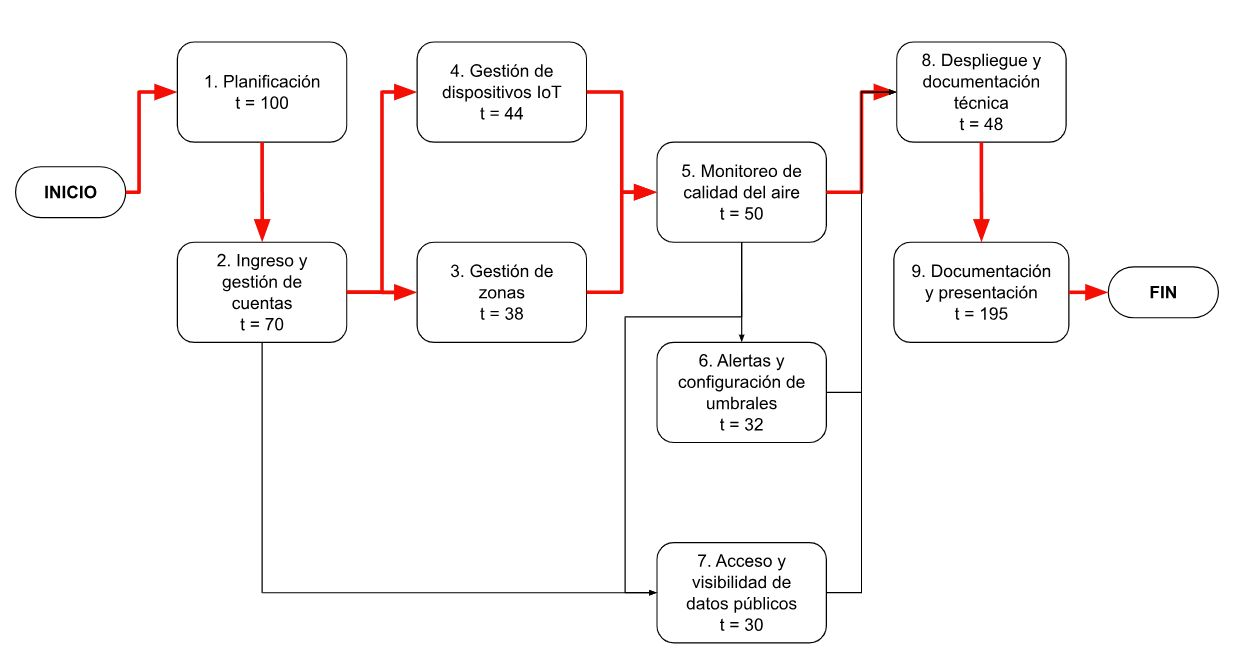
\includegraphics[width=0.7\textwidth]{./Figuras/fig_2-diagrama-AON.jpeg}
\caption{Diagrama de \textit{Activity on Node}.}
\label{fig:AoN}
\end{figure}

\begin{itemize}
    \item Las tareas están agrupadas en etapas según el desglose del trabajo en tareas.
    \item Las duraciones $t$ están expresadas en horas.
    \item Las flechas rojas indican caminos críticos parciales entre tareas dependientes.
\end{itemize}

\begin{landscape}
\section{11. Diagrama de Gantt}
\label{sec:gantt}

En la figura 3 se muestra el diagrama de Gantt general del proyecto.

\begin{figure}[htpb]
\centering 
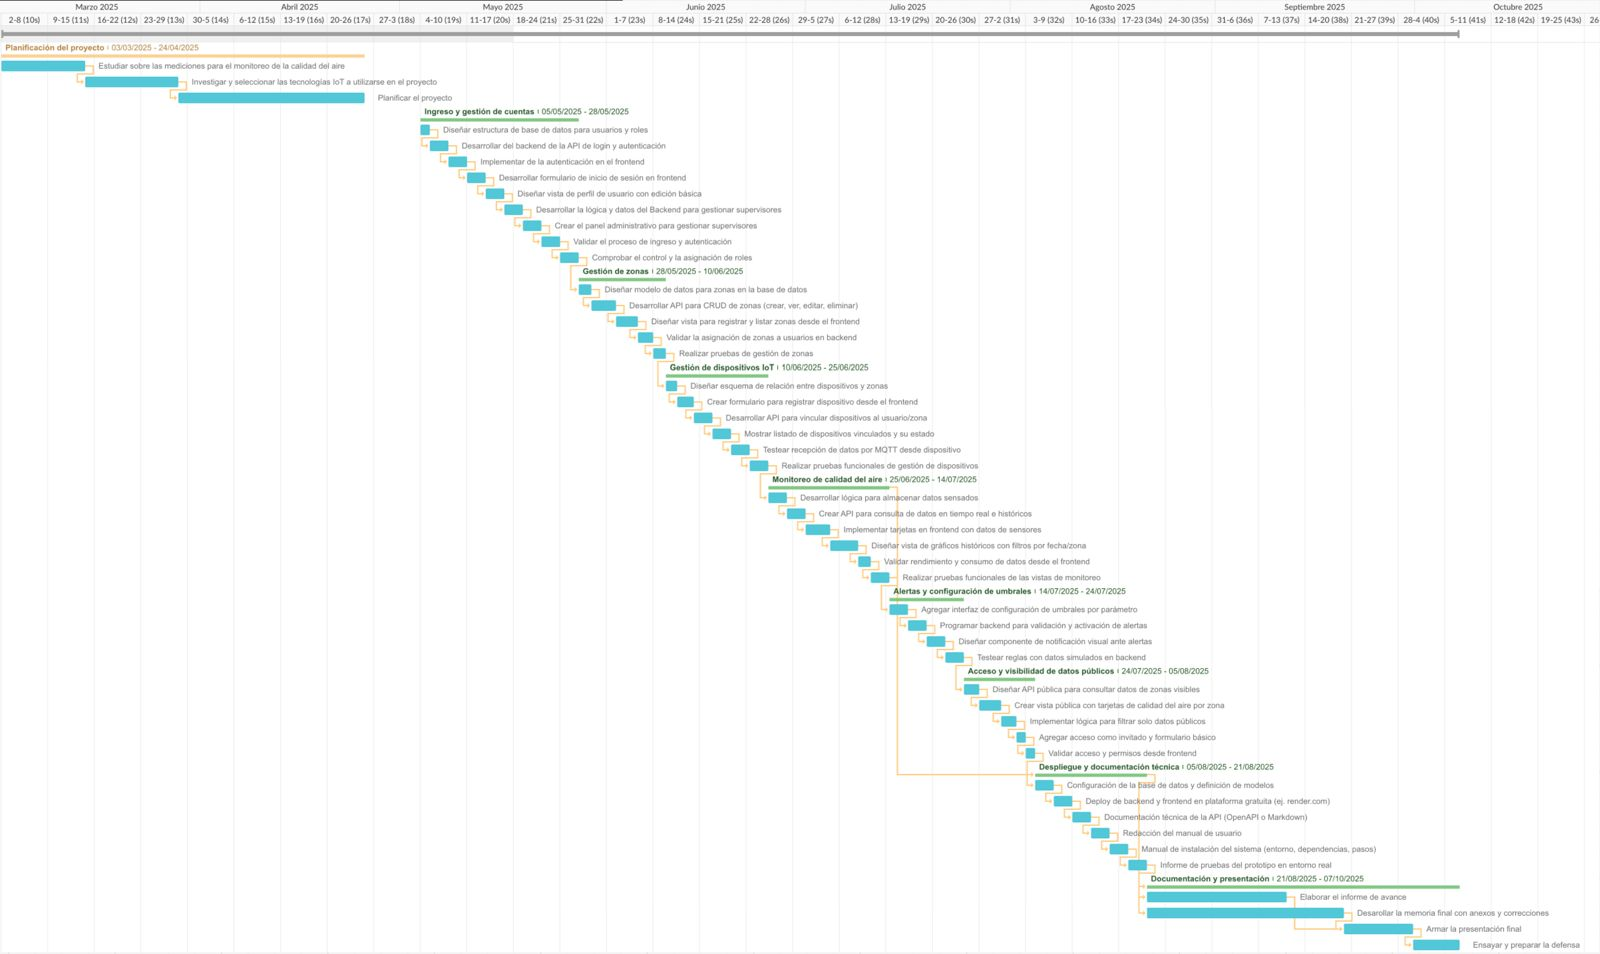
\includegraphics[width=1.2\textwidth]{./Figuras/fig_3-Gantt.jpeg}
\caption{Diagrama de Gantt del proyecto.}
\label{fig:Gantt}
\end{figure}

\end{landscape}

\section{12. Presupuesto detallado del proyecto}
\label{sec:presupuesto}

Los valores de los costos están expresados en dólares estadounidenses (USD). Al momento de elaborar el presente documento, 4 de abril del 2025, su tasa de conversión a pesos argentinos es de 1319/1 USD (referencia dólar MEP).

En la tabla 1, se visualiza un cuadro con el presupuesto del proyecto. Todas las unidades se encuentran expresadas en USD.
\begin{table}[htpb]
\centering
\begin{tabularx}{\linewidth}{@{}|X|c|r|r|@{}}
\hline
\rowcolor[HTML]{C0C0C0} 
\multicolumn{4}{|c|}{\cellcolor[HTML]{C0C0C0}COSTOS DIRECTOS} \\ \hline
\rowcolor[HTML]{C0C0C0} 
Descripción &
  \multicolumn{1}{c|}{Cantidad} &
  \multicolumn{1}{c|}{Valor unitario (USD)} &
  \multicolumn{1}{c|}{Valor total (USD)} \\ \hline
Sensor de polvo PM2.5 - PMS7003 & 3 & \$27,00 & \$81,00 \\ \hline
Sensor de gas SCD41 & 3 & \$31,00 & \$93,00 \\ \hline
Sensor CCS811 CO2 & 3 & \$12,88 & \$38,64 \\ \hline
WisGate Edge Lite 2 RAK7268V2/RAK7268CV2 & 1 & \$139,00 & \$139,00 \\ \hline
Mini UPS con salida 12VDC & 1 & \$19,00 & \$19,00 \\ \hline
ESP32 LoRa V3 + batería 1100 mAh + accesorios & 4 & \$31,50 & \$126,00 \\ \hline
Horas de trabajo & 610 & \$10,00 & \$6.100,00 \\ \hline
\multicolumn{3}{|c|}{\textbf{SUBTOTAL}} & \textbf{\$6.596,64} \\ \hline

\rowcolor[HTML]{C0C0C0} 
\multicolumn{4}{|c|}{\cellcolor[HTML]{C0C0C0}COSTOS INDIRECTOS} \\ \hline
\rowcolor[HTML]{C0C0C0} 
Descripción &
  \multicolumn{1}{c|}{Cantidad} &
  \multicolumn{1}{c|}{Valor unitario (USD)} &
  \multicolumn{1}{c|}{Valor total (USD)} \\ \hline
30\% sobre costos directos & 1 & \$1.978,99 & \$1.978,99 \\ \hline
\multicolumn{3}{|c|}{\textbf{SUBTOTAL}} & \textbf{\$1.978,99} \\ \hline
\rowcolor[HTML]{C0C0C0}
\multicolumn{3}{|c|}{\textbf{TOTAL}} & \textbf{\$8.575,63} \\ \hline
\end{tabularx}
\caption{Presupuesto detallado del proyecto.}
\label{tab:presupuesto}
\end{table}



\section{13. Gestión de riesgos}
\label{sec:riesgos}

\subsection*{a) Identificación de los riesgos y estimación de consecuencias}

Riesgo 1: fallo en la comunicación entre los dispositivos IoT y el servidor

\begin{itemize}
	\item Severidad (S): 8\\
	Una interrupción en la comunicación impide la recolección de datos en tiempo real, afectando la utilidad del sistema para el monitoreo ambiental.
	\item Ocurrencia (O): 6\\
	Existe una probabilidad media-alta de ocurrencia debido a interferencias o problemas de cobertura en redes WiFi o LoRaWAN durante el prototipo.
\end{itemize}

Riesgo 2: sobrecarga de recursos en los dispositivos IoT

\begin{itemize}
	\item Severidad (S): 8.\\
	Si un nodo falla de forma inesperada, se pierde la continuidad del monitoreo, y puede interrumpirse la cadena de datos.
	\item Ocurrencia (O): 6.\\
	El ESP32, aunque potente, tiene limitaciones en RAM y CPU. Cargar múltiples sensores, comunicaciones paralelas y lógica de validación sin optimización puede llevar al cuelgue o reinicio del dispositivo.
\end{itemize}

Riesgo 3: problemas de compatibilidad entre sensores y microcontrolador

\begin{itemize}
	\item Severidad (S): 6.\\
	Podría afectar la calidad de los datos o requerir modificaciones de hardware/software no planificadas.
	\item Ocurrencia (O): 5.\\
	Se eligieron sensores compatibles, pero pueden presentarse inconsistencias en las librerías o el consumo de energía.
\end{itemize}

Riesgo 4: saturación o malformación de datos sensados

\begin{itemize}
	\item Severidad (S): 7.\\
	La mala interpretación de datos puede activar alertas falsas o provocar decisiones erróneas.
	\item Ocurrencia (O): 6.\\
	Es un riesgo común en sensores ambientales económicos o mal configurados.
\end{itemize}

Riesgo 5: fallo de los servicios de despliegue gratuito

\begin{itemize}
	\item Severidad (S): 7.\\
	Una interrupción del entorno de ejecución \textit{cloud} o local durante una instancia crítica como pruebas, comprometería la validación del sistema en tiempo real.
	\item Ocurrencia (O): 5.\\
	Si bien los entornos pueden ser robustos, los errores de configuración, las restricciones presupuestarias en servicios \textit{cloud} gratuitos, o incluso errores en el runtime pueden generar indisponibilidad momentánea.
\end{itemize}

\subsection*{b) Tabla de gestión de riesgos}

\begin{table}[htpb]
\centering
\begin{tabularx}{\linewidth}{@{}|X|c|c|c|c|c|c|@{}}
\hline
\rowcolor[HTML]{C0C0C0} 
\textbf{Riesgo} & \textbf{S} & \textbf{O} & \textbf{RPN} & \textbf{S*} & \textbf{O*} & \textbf{RPN*} \\ \hline
Fallo en comunicación IoT-servidor & 8 & 6 & 48 & 6 & 4 & 24 \\ \hline
Sobrecarga de recursos en los dispositivos IoT & 8 & 6 & 48 & 6 & 4 & 24 \\ \hline
Compatibilidad entre sensores y microcontrolador & 6 & 5 & 30 & 5 & 4 & 20 \\ \hline
Saturación o malformación de datos sensados & 7 & 6 & 42 & 5 & 3 & 15 \\ \hline
Fallo del servicio Render.com & 7 & 5 & 35 & 5 & 3 & 15 \\ \hline
\end{tabularx}
\caption{Evaluación de riesgos antes y después de la mitigación.}
\end{table}

Criterio adoptado: Se tomarán medidas de mitigación para todos los riesgos con RPN inicial mayor a 25. \\
Nota: los valores marcados con (*) en la tabla corresponden luego de haber aplicado la mitigación.


\subsection*{c) Plan de mitigación}

Riesgo 1: fallo en la comunicación IoT-servidor

Plan de mitigación: incluir mecanismos de reintento automático, logs de errores y pruebas en distintos entornos para validar la conectividad. Asegurar compatibilidad entre MQTT y LoRaWAN mediante brokers intermedios.

\begin{itemize}
	\item Severidad (S*): 6.\\ Se redujo al contar con validaciones de conectividad y almacenamiento temporal local.
	\item Ocurrencia (O*): 4.\\ Disminuye al hacer pruebas exhaustivas y usar hardware probado.
\end{itemize}

Riesgo 2: sobrecarga de recursos en los dispositivos IoT

Plan de mitigación: planificar tareas pequeñas, usar recursos de aprendizaje continuo y apoyo con herramientas de depuración. Reutilizar plantillas y librerías probadas.

\begin{itemize}
	\item Severidad (S*): 6.\\
	Con mecanismos de autorrecuperación, el impacto se reduce.
	\item Ocurrencia (O*): 4.\\
	La probabilidad disminuye al optimizar el uso de memoria y mantener lógica desacoplada.
\end{itemize}

Riesgo 3: compatibilidad sensores - microcontrolador

Plan de mitigación: testeo unitario anticipado y validación con ejemplos oficiales de MicroPython y C/C++. Uso de fuentes de alimentación externa para sensores que lo requieran.

\begin{itemize}
	\item Severidad (S*): 5.\\ El riesgo técnico se reduce con pruebas en laboratorio.
	\item Ocurrencia (O*): 4.\\ Menor al contar con documentación adecuada y soporte de comunidad.
\end{itemize}

Riesgo 4: saturación o malformación de datos sensados

Plan de mitigación: aplicar filtros de validación de rango en el \textit{firmware} (por ejemplo, descartar valores extremos o “nan”), así como lógica de suavizado o \textit{debounce} de señales antes de que lleguen al \textit{backend}.

\begin{itemize}
	\item Severidad (S*): 5.\\
	Con validación previa se evita que el dato incorrecto afecte la plataforma.
	\item Ocurrencia (O*): 3.\\
	La probabilidad se reduce si se validan lecturas en \textit{firmware} + \textit{backend}.
\end{itemize}
Riesgo 5: Fallo del servicio

Plan de mitigación: contar con una versión Dockerizada funcional del sistema que pueda ejecutarse localmente sin conexión a internet. Además, mantener backups de configuración en distintos proveedores y realizar ensayos de contingencia antes de la presentación.

\begin{itemize}
	\item Severidad (S*): 5.\\
	El impacto se reduce al poder replicar la arquitectura localmente sin depender del servicio externo.
	\item Ocurrencia (O*): 3.\\
	La probabilidad disminuye al tener redundancia y pruebas previas del entorno final.
\end{itemize}

\section{14. Gestión de la calidad}
\label{sec:calidad}

A continuación, se detallan los requerimientos considerados críticos o de alto valor para el cumplimiento del objetivo del sistema, junto con sus acciones de verificación y validación.


\begin{itemize}
	\item Req \# 1: el sistema deberá capturar datos ambientales a través de sensores conectados a dispositivos IoT.

    \begin{itemize}
	    \item Verificación: se probará cada sensor en condiciones controladas, comparando los valores con instrumentos de referencia o condiciones conocidas. Se revisará el \textit{firmware} del ESP32 para verificar que realiza lecturas correctas.
	    \item Validación: se observará el comportamiento del sistema desde la interfaz web, verificando que los datos se actualizan en condiciones cambiantes (por ejemplo, al acercar una fuente de calor o CO2).
    \end{itemize}

	\item Req \# 2: el sistema deberá enviar los datos al servidor en tiempo real utilizando WiFi o LoRa/MQTT
	\begin{itemize}
		\item Verificación: se analizarán los paquetes enviados con herramientas como MQTT.fx o Mosquitto CLI, asegurando su frecuencia y estructura.
		\item Validación: se revisará en el panel de usuario que los datos se actualicen en tiempo real tras un evento medible.
	\end{itemize}
	
	\item Req \# 3: El sistema deberá almacenar los datos para su posterior análisis.
	\begin{itemize}
		\item Verificación: se inspeccionará directamente la base de datos para confirmar la correcta inserción de datos con marcas de tiempo y relaciones válidas.

		\item Validación: se utilizará la interfaz para seleccionar un rango de fechas y verificar que se presentan correctamente los datos históricos.
	\end{itemize}

	\item Req \# 4: Se deberá ofrecer la opción de publicar los datos como privados o públicos.
	\begin{itemize}
		\item Verificación: se revisará el \textit{backend} para asegurar que se respeta el parámetro de visibilidad, y que la lógica de autorización limita el acceso a los datos según el estado de cada sensor o zona.
		\item Validación: se probará la vista de invitado y se comprobará que no accede a datos privados.
	\end{itemize}
	
	\item Req \# 5: El sistema deberá generar alertas si se superan umbrales definidos como peligrosos.
	\begin{itemize}
		\item Verificación: se forzarán lecturas fuera de rango para comprobar que la lógica de alertas se activa correctamente en el \textit{backend}.
		\item Validación: se observará en la interfaz que se muestra una alerta clara y comprensible, con el parámetro afectado y el valor medido.
	\end{itemize}
	
	\item Req \# 6: La plataforma deberá contar con una interfaz web responsiva.
	\begin{itemize}
		\item Verificación: se realizarán pruebas en múltiples resoluciones usando herramientas de desarrollo y emuladores, verificando adaptabilidad de cada componente.
		\item Validación: se accederá a la plataforma desde distintos dispositivos y se confirmará con el usuario que la experiencia de uso es adecuada.
	\end{itemize}
	
	\item Req \# 7: Los indicadores de calidad del aire deberán representarse mediante códigos de colores.
	\begin{itemize}
		\item Verificación: se revisará la lógica del frontend para confirmar que los colores asignados se corresponden con los rangos establecidos en normativa.
		\item Validación: el usuario verá un panel que indique visualmente, por color, el estado ambiental de cada zona.
	\end{itemize}
	
	\item Req \# 8: El usuario deberá poder registrar, editar y eliminar zonas de monitoreo.
	\begin{itemize}
		\item Verificación: se probarán los \textit{endpoints} de la API para operaciones CRUD en zonas y su impacto en la base de datos.
		\item Validación: se confirmará, desde la interfaz, que se puede realizar la gestión de zonas sin errores, y que los cambios se reflejan inmediatamente.
	\end{itemize}
	
	\item Req \# 9: El sistema deberá ejecutarse en un entorno Dockerizado portátil.
	\begin{itemize}
		\item Verificación: se construirá y ejecutará una imagen Docker del sistema, verificando su correcto funcionamiento desde CLI y logs del contenedor.
		\item Validación: el contenedor se compartirá con un tercero para validar que el entorno puede reproducirse sin errores adicionales.
	\end{itemize}
	
	\item Req \# 10: El visitante podrá visualizar datos públicos sin necesidad de registrarse.
	\begin{itemize}
		\item Verificación: se analizará el \textit{backend} y las consultas para comprobar que no se requiere token y que sólo se retornan datos públicos.
		\item Validación: como invitado, se accederá a la vista pública y se confirmará que los datos se muestran correctamente y están limitados a la visibilidad asignada.
	\end{itemize}

\end{itemize}

\section{15. Procesos de cierre}    
\label{sec:cierre}

Una vez concluido el proyecto, se establecerán las siguientes pautas de trabajo que permitirán evaluar su ejecución, registrar aprendizajes y agradecer la colaboración de los distintos interesados:

\begin{itemize}
	\item Análisis del cumplimiento del Plan de Proyecto original: \\
	\begin{itemize}
		\item A cargo del {\authorname}, {\clientename} y {\supname} se revisará si las actividades definidas se completaron en los tiempos y alcances planificados. Se utilizará como referencia el diagrama de Gantt y los registros de avances documentados durante el desarrollo.
		\item Se elaborará una síntesis comparativa entre lo planificado y lo realmente ejecutado, con observaciones sobre desviaciones y justificaciones correspondientes.
		\item Este análisis será incluido en el informe final y presentado durante la reunión de cierre.
		\item 
    \end{itemize}		
	   

	\item Identificación de técnicas útiles, problemas y soluciones aplicadas:  \\
	El {\authorname} también será responsable de redactar un informe reflexivo donde se detallen:
	\begin{itemize}
	    \item Las herramientas, tecnologías y metodologías que resultaron más eficaces para el desarrollo (por ejemplo, uso de Docker, modularización del backend, visualización en tiempo real).
	    \item Aquellas que no aportaron valor o que presentaron dificultades significativas.
	    \item Los principales problemas encontrados (como fallos en sensores o restricciones de conectividad) y las soluciones implementadas. 
	\end{itemize}
	Esta documentación quedará como anexo del proyecto y será publicada junto al repositorio para referencia futura.

	\item Agradecimiento a interesados y colaboradores:  \\
	\begin{itemize}
	\item El {\authorname} se encargará de organizar el acto simbólico de agradecimiento a quienes participaron directa o indirectamente del proyecto, especialmente al director del trabajo final, al docente responsable, y a quienes brindaron apoyo técnico o institucional.  
	\item Esta actividad se realizará al finalizar la defensa del proyecto, incluyendo un breve mensaje público y mención especial en la memoria. No se contemplan gastos financieros significativos, por lo que no se requiere asignación presupuestaria específica.
    \end{itemize}		
	
\end{itemize}


\end{document}
